% Ubah judul dan label berikut sesuai dengan yang diinginkan.
\section{System Design and Implementation}
\label{sec:designandimplementation}

\subsection{System Architecture Overview}

The proposed system implements a comprehensive approach to overdimension vehicle detection through a sophisticated three-tier architecture. At its foundation, the Edge Processing Layer handles real-time video capture and processing, leveraging optimized models for on-device inference while maintaining local data buffering and preprocessing capabilities. This is complemented by a robust Cloud Infrastructure that provides centralized data storage and management, coupled with authentication and authorization services, alongside comprehensive analytics and reporting capabilities. The system's user interface is delivered through a Mobile Interface component, featuring a real-time monitoring dashboard, push notification system, and historical data access functionality.

\begin{figure}[htbp]
  \centering
  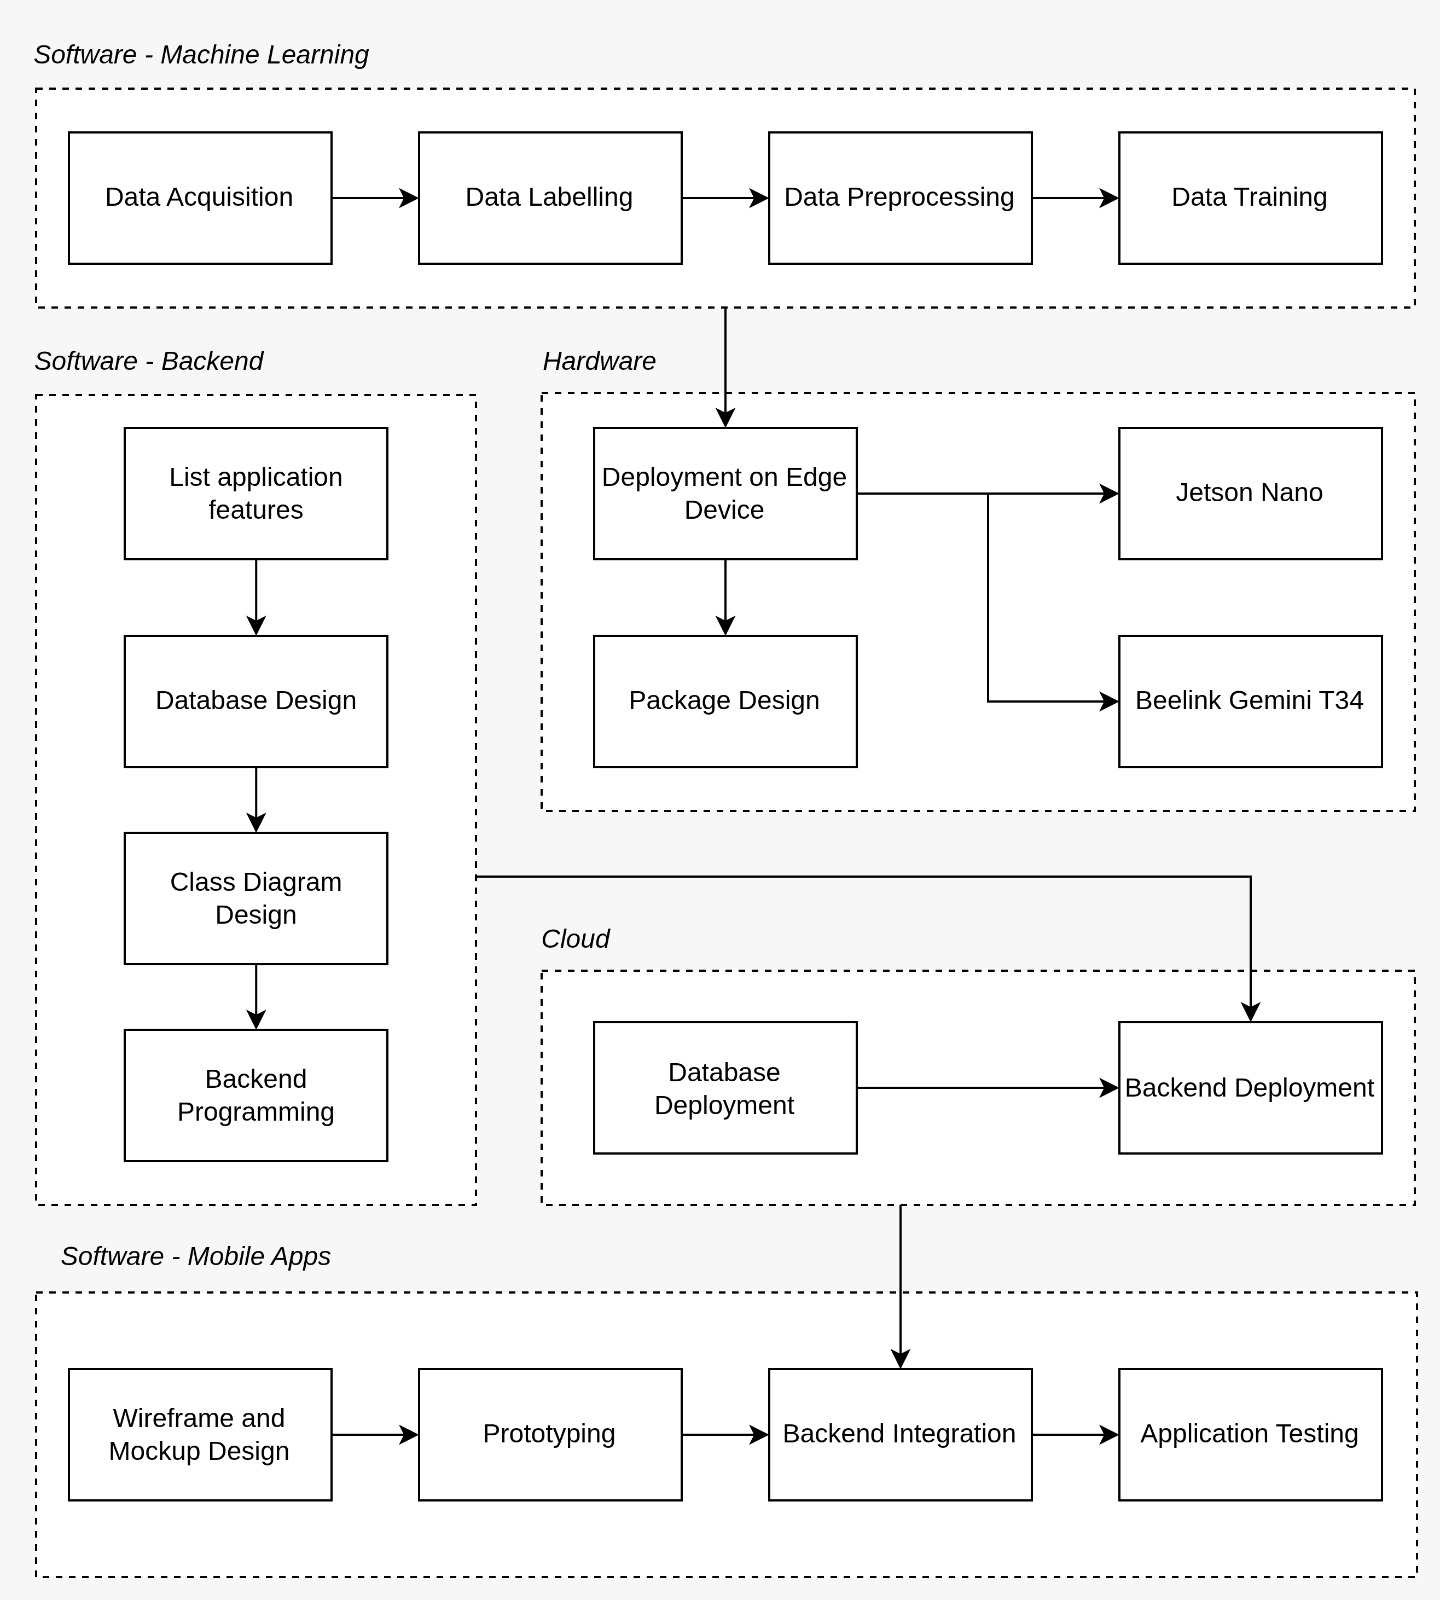
\includegraphics[scale=0.15]{gambar/bab3-block-diagram-en.jpeg}
  \caption{System Architecture Overview}
  \label{fig:arsitektur_sistem}
\end{figure}

\subsection{Detection Model Development}

\subsubsection{Dataset Preparation}
The development of a robust detection model began with meticulous dataset curation and augmentation. The initial collection of images was enhanced through various augmentation techniques, resulting in a comprehensive dataset of 823 images encompassing diverse scenarios including varied lighting conditions, multiple vehicle angles, and different traffic situations. The data processing pipeline involved standardizing image resolutions to 300×300 pixels, applying augmentation techniques such as rotation, scaling, and brightness adjustments, and implementing class balancing measures. The augmented dataset was strategically split for training and validation, with a separate test set of 166 images reserved for final performance evaluation, ensuring a thorough assessment of the model's real-world capabilities.

\subsubsection{Model Configuration}
The SSD-MobileNetV2 model underwent extensive optimization through careful parameter tuning and architectural refinements. Training configurations explored both 30 and 50 epoch scenarios, utilizing a batch size of 16. Two learning rate schedulers were evaluated: CosineAnnealingLR for smooth convergence characteristics and MultiStepLR for comparative analysis. The model architecture was built around a MobileNetV2 backbone for feature extraction, complemented by an SSD detection head with multiple scales, and specialized output layers for class prediction and bounding box regression.

\subsection{Edge Device Implementation}

\subsubsection{Hardware Specifications}
The system's edge computing capabilities were evaluated across two distinct platforms, each offering unique performance characteristics. The NVIDIA Jetson Nano, featuring a quad-core ARM A57 processor running at 1.43 GHz and a 128-core Maxwell architecture GPU, provides 4GB of LPDDR4 memory operating at 1600 MHz, complemented by 16GB of eMMC 5.1 storage. This configuration maintains an efficient power consumption profile of 5-10W. In contrast, the Beelink Gemini T34 offers an Intel Celeron N3350 processor operating at 2.4 GHz, supported by 8GB of DDR4 RAM and 128GB SSD storage, with a power consumption range of 10-15W.

\subsubsection{Software Stack}
The implementation leverages a carefully selected stack of optimized frameworks to ensure optimal performance. The core components are built upon Ubuntu 20.04 LTS as the operating system, incorporating PyTorch 1.9 for deep learning operations, OpenCV 4.5 for video processing tasks, and TensorRT 8.0 for model optimization. Custom software components include a sophisticated detection pipeline manager, specialized data preprocessing modules, robust communication interfaces, and comprehensive system monitoring tools, all designed to work in harmony for efficient system operation.

\subsection{Cloud Infrastructure}

\subsubsection{Backend Services}
The cloud system architecture provides a comprehensive suite of services designed for optimal performance and reliability. Core services encompass real-time data storage and retrieval capabilities, robust user authentication and authorization mechanisms, well-documented REST API endpoints for client communication, and an automated notification dispatch system. The data management infrastructure is built around a PostgreSQL database for structured data storage, complemented by object storage for detection images, an efficient cache layer for enhanced performance, and automated backup systems ensuring data integrity and availability.

\subsection{Mobile Application Development}

\subsubsection{Technical Implementation}
The mobile application, developed using Flutter, represents a sophisticated client-side solution with comprehensive functionality. Core features include real-time detection monitoring capabilities, an advanced push notification system, intuitive historical data visualization tools, and streamlined user profile management. The application's architecture follows industry best practices, implementing the BLoC pattern for state management, utilizing the repository pattern for data access, incorporating a service layer for API communication, and maintaining local storage capabilities for offline functionality.

\subsection{Testing Methodology}

\subsubsection{Performance Evaluation}
The testing strategy encompassed a comprehensive evaluation across multiple dimensions of system performance. Model evaluation focused on key metrics including accuracy measurements through mAP calculations, inference speed monitoring in FPS, detailed resource utilization analysis, and overall detection reliability assessment. System testing extended to end-to-end integration verification, network performance evaluation, data synchronization validation, and thorough error handling assessment. The user interface underwent rigorous testing for responsiveness, feature accessibility, cross-platform compatibility, and various user experience metrics.

\subsubsection{Deployment Strategy}
The implementation followed a carefully structured phased approach to ensure system reliability and performance. Phase 1 focused on thorough laboratory testing and optimization procedures. Phase 2 involved controlled environment deployment to validate system behavior under specific conditions. Phase 3 expanded to limited field trials, gathering real-world performance data. Finally, Phase 4 culminated in full-scale implementation, incorporating lessons learned from previous phases to ensure optimal system operation.